
% Appendix  A %%%%%%%%%%%%%%%%%%%%%%%%%%%%%%
\begin{landscape}
\hypertarget{aggregated-data}{%
\section{Supplementary Tables}\label{aggregated-data}}
\renewcommand{\arraystretch}{0.8}% Tighter

\begingroup\fontsize{7}{9}\selectfont

\begin{ThreePartTable}
\begin{TableNotes}
\item \textit{Notes: } 
\item Education reports mean (sd); IR(G) reports inequality ratios between the group with the highest and lowest average education.
\end{TableNotes}
\begin{longtable}[t]{lccccccc}
\caption{\label{tab:aggregated}Education Inequality Ratios by Birth Cohort and Country for Gender and Ethnicity}\\
\toprule
Cohort & Education & IR(gender) & IR(eth) & IR(gen:eth) & IR(gen:eth)' & Differential & obs.\\
\midrule
\endfirsthead
\caption[]{Education Inequality Ratios by Birth Cohort and Country for Gender and Ethnicity \textit{(continued)}}\\
\toprule
Cohort & Education & IR(gender) & IR(eth) & IR(gen:eth) & IR(gen:eth)' & Differential & obs.\\
\midrule
\endhead

\endfoot
\bottomrule
\insertTableNotes
\endlastfoot
\addlinespace[0.3em]
\multicolumn{8}{l}{\textbf{Afghanistan}}\\
\hspace{1em}1970-1979 & 1.6 (3.62) & 0.81 & 0.63 & 0.99 & 0.93 & 0.07 & 10207\\
\hspace{1em}1980- & 2 (3.94) & 0.77 & 0.66 & 0.97 & 0.92 & 0.05 & 17528\\
\addlinespace[0.3em]
\multicolumn{8}{l}{\textbf{Albania}}\\
\hspace{1em}-1969 & 11.37 (4.04) & 0.06 & 0.21 & 0.27 & 0.26 & 0.01 & 10061\\
\hspace{1em}1970-1979 & 11.35 (4) & 0.01 & 0.25 & 0.30 & 0.25 & 0.04 & 7103\\
\hspace{1em}1980- & 12.14 (4.64) & 0.06 & 0.38 & 0.44 & 0.42 & 0.02 & 6443\\
\addlinespace[0.3em]
\multicolumn{8}{l}{\textbf{Benin}}\\
\hspace{1em}-1969 & 2.33 (4.06) & 0.54 & 0.93 & 0.97 & 0.97 & 0.01 & 17112\\
\hspace{1em}1970-1979 & 2.19 (3.7) & 0.56 & 0.85 & 0.94 & 0.94 & 0.01 & 19084\\
\hspace{1em}1980- & 2.86 (4.51) & 0.55 & 0.82 & 0.94 & 0.92 & 0.02 & 17737\\
\addlinespace[0.3em]
\multicolumn{8}{l}{\textbf{Bolivia}}\\
\hspace{1em}-1969 & 6.78 (5.1) & 0.17 & 0.33 & 0.43 & 0.45 & -0.02 & 8613\\
\hspace{1em}1970-1979 & 8.57 (4.92) & 0.17 & 0.24 & 0.35 & 0.36 & -0.02 & 6097\\
\addlinespace[0.3em]
\multicolumn{8}{l}{\textbf{Brazil}}\\
\hspace{1em}-1969 & 6.13 (4.23) & 0.08 & 0.25 & 0.32 & 0.31 & 0.01 & 9031\\
\hspace{1em}1970-1979 & 6.94 (3.88) & 0.11 & 0.17 & 0.34 & 0.27 & 0.07 & 894\\
\addlinespace[0.3em]
\multicolumn{8}{l}{\textbf{Burkina Faso}}\\
\hspace{1em}-1969 & 0.92 (2.8) & 0.50 & 0.76 & 0.90 & 0.88 & 0.02 & 18787\\
\hspace{1em}1970-1979 & 1.54 (3.52) & 0.56 & 0.76 & 0.89 & 0.90 & -0.01 & 11479\\
\hspace{1em}1980- & 1.96 (3.78) & 0.47 & 0.83 & 0.94 & 0.91 & 0.02 & 4883\\
\addlinespace[0.3em]
\multicolumn{8}{l}{\textbf{Cameroon}}\\
\hspace{1em}-1969 & 5.24 (4.54) & 0.31 & 0.89 & 0.95 & 0.93 & 0.03 & 13493\\
\hspace{1em}1970-1979 & 6.27 (4.58) & 0.25 & 0.79 & 0.91 & 0.84 & 0.06 & 13365\\
\hspace{1em}1980- & 7 (4.99) & 0.22 & 0.76 & 0.83 & 0.81 & 0.03 & 12775\\
\addlinespace[0.3em]
\multicolumn{8}{l}{\textbf{Central African Republic}}\\
\hspace{1em}-1969 & 2.45 (3.64) & 0.58 & 0.78 & 0.93 & 0.91 & 0.03 & 4616\\
\addlinespace[0.3em]
\multicolumn{8}{l}{\textbf{Chad}}\\
\hspace{1em}-1969 & 1.19 (2.84) & 0.72 & 0.87 & 0.98 & 0.96 & 0.02 & 9039\\
\hspace{1em}1970-1979 & 1.61 (3.3) & 0.70 & 0.83 & 0.96 & 0.95 & 0.01 & 7536\\
\hspace{1em}1980- & 2.44 (3.97) & 0.61 & 0.87 & 0.95 & 0.95 & 0.00 & 7733\\
\addlinespace[0.3em]
\multicolumn{8}{l}{\textbf{Congo}}\\
\hspace{1em}-1969 & 8.13 (4.38) & 0.28 & 0.34 & 0.52 & 0.53 & 0.00 & 5256\\
\hspace{1em}1970-1979 & 8.2 (3.75) & 0.19 & 0.19 & 0.38 & 0.35 & 0.03 & 7173\\
\hspace{1em}1980- & 8.32 (3.85) & 0.11 & 0.32 & 0.45 & 0.40 & 0.05 & 3930\\
\addlinespace[0.3em]
\multicolumn{8}{l}{\textbf{DR Congo}}\\
\hspace{1em}-1969 & 6.28 (4.59) & 0.46 & 0.43 & 0.70 & 0.69 & 0.01 & 6636\\
\hspace{1em}1970-1979 & 6.55 (4.45) & 0.35 & 0.39 & 0.56 & 0.61 & -0.05 & 9335\\
\hspace{1em}1980- & 6.59 (4.58) & 0.34 & 0.38 & 0.57 & 0.59 & -0.02 & 9355\\
\addlinespace[0.3em]
\multicolumn{8}{l}{\textbf{Ethiopia}}\\
\hspace{1em}-1969 & 1.48 (3.35) & 0.68 & 0.90 & NaN & 0.97 & NaN & 17072\\
\hspace{1em}1970-1979 & 2.34 (3.92) & 0.49 & 0.88 & 0.99 & 0.94 & 0.05 & 20654\\
\hspace{1em}1980- & 3.42 (4.69) & 0.51 & 0.82 & 0.97 & 0.91 & 0.05 & 18944\\
\addlinespace[0.3em]
\multicolumn{8}{l}{\textbf{Gabon}}\\
\hspace{1em}-1969 & 8.6 (3.8) & 0.24 & 0.29 & 0.58 & 0.46 & 0.13 & 2079\\
\hspace{1em}1970-1979 & 9.03 (3.87) & 0.20 & 0.33 & 0.49 & 0.46 & 0.03 & 2680\\
\hspace{1em}1980- & 9.81 (3.82) & 0.11 & 0.21 & 0.32 & 0.29 & 0.03 & 2506\\
\addlinespace[0.3em]
\multicolumn{8}{l}{\textbf{Ghana}}\\
\hspace{1em}-1969 & 6.14 (5.18) & 0.34 & 0.84 & 0.89 & 0.90 & 0.00 & 11024\\
\hspace{1em}1970-1979 & 6.88 (5.03) & 0.28 & 0.68 & 0.85 & 0.77 & 0.08 & 6505\\
\hspace{1em}1980- & 8.27 (5.17) & 0.18 & 0.64 & 0.74 & 0.70 & 0.04 & 5177\\
\addlinespace[0.3em]
\multicolumn{8}{l}{\textbf{Guatemala}}\\
\hspace{1em}-1969 & 4.26 (4.7) & 0.24 & 0.58 & 0.73 & 0.68 & 0.06 & 3783\\
\hspace{1em}1970-1979 & 4.92 (4.74) & 0.20 & 0.51 & 0.63 & 0.61 & 0.02 & 7471\\
\hspace{1em}1980- & 6.38 (4.9) & 0.15 & 0.42 & 0.50 & 0.50 & 0.00 & 10798\\
\addlinespace[0.3em]
\multicolumn{8}{l}{\textbf{Guinea}}\\
\hspace{1em}-1969 & 1.77 (4.24) & 0.62 & 0.62 & 0.84 & 0.86 & -0.01 & 4734\\
\hspace{1em}1970-1979 & 1.64 (3.95) & 0.72 & 0.58 & 0.88 & 0.88 & 0.00 & 4253\\
\hspace{1em}1980- & 3.03 (5.29) & 0.60 & 0.59 & 0.82 & 0.84 & -0.02 & 5811\\
\addlinespace[0.3em]
\multicolumn{8}{l}{\textbf{Guyana}}\\
\hspace{1em}-1969 & 7.92 (3.39) & 0.03 & 0.34 & 0.39 & 0.36 & 0.02 & 2065\\
\hspace{1em}1970-1979 & 8.64 (3.28) & 0.05 & 0.35 & 0.38 & 0.38 & 0.00 & 2327\\
\hspace{1em}1980- & 9.26 (3.09) & 0.00 & 0.32 & 0.39 & 0.32 & 0.06 & 1118\\
\addlinespace[0.3em]
\multicolumn{8}{l}{\textbf{Honduras}}\\
\hspace{1em}-1969 & 5.66 (4.57) & 0.11 & 0.39 & 0.54 & 0.46 & 0.08 & 4657\\
\hspace{1em}1970-1979 & 6.44 (4.3) & 0.06 & 0.32 & 0.38 & 0.37 & 0.01 & 7036\\
\hspace{1em}1980- & 7.51 (4.34) & 0.09 & 0.29 & 0.37 & 0.35 & 0.02 & 6768\\
\addlinespace[0.3em]
\multicolumn{8}{l}{\textbf{Ivory Coast}}\\
\hspace{1em}-1969 & 2.4 (3.91) & 0.53 & 0.76 & 0.91 & 0.89 & 0.03 & 6088\\
\addlinespace[0.3em]
\multicolumn{8}{l}{\textbf{Kazakhstan}}\\
\hspace{1em}-1969 & 10.77 (2.51) & 0.15 & 0.04 & 0.20 & 0.18 & 0.02 & 3533\\
\hspace{1em}1970-1979 & 10.77 (2.24) & 0.16 & 0.03 & 0.19 & 0.18 & 0.00 & 875\\
\addlinespace[0.3em]
\multicolumn{8}{l}{\textbf{Kenya}}\\
\hspace{1em}-1969 & 6.55 (4.3) & 0.25 & 0.84 & 0.93 & 0.88 & 0.05 & 19245\\
\hspace{1em}1970-1979 & 8.16 (3.94) & 0.13 & 0.80 & 0.88 & 0.83 & 0.05 & 18720\\
\hspace{1em}1980- & 8.84 (3.99) & 0.09 & 0.75 & 0.84 & 0.77 & 0.07 & 15797\\
\addlinespace[0.3em]
\multicolumn{8}{l}{\textbf{Liberia}}\\
\hspace{1em}-1969 & 4.39 (5.16) & 0.65 & 0.45 & 0.82 & 0.80 & 0.02 & 1402\\
\hspace{1em}1970-1979 & 4.55 (5.01) & 0.49 & 0.43 & 0.71 & 0.71 & 0.00 & 3187\\
\hspace{1em}1980- & 5.59 (5.12) & 0.36 & 0.31 & 0.63 & 0.56 & 0.07 & 3776\\
\addlinespace[0.3em]
\multicolumn{8}{l}{\textbf{Malawi}}\\
\hspace{1em}-1969 & 3.63 (3.65) & 0.40 & 0.66 & 0.84 & 0.80 & 0.04 & 15246\\
\hspace{1em}1970-1979 & 4.56 (3.96) & 0.34 & 0.56 & 0.72 & 0.71 & 0.02 & 21043\\
\hspace{1em}1980- & 6.32 (3.89) & 0.17 & 0.35 & 0.47 & 0.46 & 0.01 & 17567\\
\addlinespace[0.3em]
\multicolumn{8}{l}{\textbf{Mali}}\\
\hspace{1em}-1969 & 1.29 (3.11) & 0.53 & 0.66 & 0.88 & 0.84 & 0.03 & 21039\\
\hspace{1em}1970-1979 & 1.3 (3.2) & 0.54 & 0.62 & 0.84 & 0.83 & 0.01 & 15553\\
\hspace{1em}1980- & 2.01 (3.99) & 0.54 & 0.67 & 0.85 & 0.85 & 0.00 & 12203\\
\addlinespace[0.3em]
\multicolumn{8}{l}{\textbf{Moldova}}\\
\hspace{1em}-1969 & 11.5 (2.33) & 0.03 & 0.07 & 0.10 & 0.10 & 0.00 & 4121\\
\hspace{1em}1970-1979 & 11.54 (2.52) & 0.01 & 0.03 & 0.04 & 0.04 & 0.00 & 2320\\
\hspace{1em}1980- & 11.78 (2.74) & 0.02 & 0.09 & 0.11 & 0.10 & 0.01 & 258\\
\addlinespace[0.3em]
\multicolumn{8}{l}{\textbf{Mozambique}}\\
\hspace{1em}-1969 & 2.21 (2.94) & 0.53 & 0.83 & 0.89 & 0.92 & -0.03 & 8073\\
\hspace{1em}1970-1979 & 3.09 (3.49) & 0.38 & 0.82 & 0.87 & 0.89 & -0.02 & 5241\\
\hspace{1em}1980- & 3.96 (3.93) & 0.35 & 0.80 & 0.85 & 0.87 & -0.02 & 3993\\
\addlinespace[0.3em]
\multicolumn{8}{l}{\textbf{Namibia}}\\
\hspace{1em}-1969 & 6.57 (4.24) & 0.02 & 0.46 & 0.53 & 0.46 & 0.07 & 3882\\
\hspace{1em}1970-1979 & 8.11 (3.76) & 0.06 & 0.38 & 0.44 & 0.41 & 0.02 & 1868\\
\addlinespace[0.3em]
\multicolumn{8}{l}{\textbf{Niger}}\\
\hspace{1em}-1969 & 0.61 (2.15) & 0.40 & 0.82 & 0.88 & 0.90 & -0.01 & 13895\\
\hspace{1em}1970-1979 & 1.18 (2.83) & 0.54 & 0.73 & 0.85 & 0.88 & -0.03 & 4970\\
\hspace{1em}1980- & 1.17 (2.91) & 0.62 & 0.71 & 0.90 & 0.89 & 0.01 & 1142\\
\addlinespace[0.3em]
\multicolumn{8}{l}{\textbf{Nigeria}}\\
\hspace{1em}-1969 & 5.51 (5.68) & 0.37 & 0.90 & 0.95 & 0.94 & 0.02 & 18869\\
\hspace{1em}1970-1979 & 6.44 (5.69) & 0.30 & 0.89 & 0.94 & 0.92 & 0.02 & 35890\\
\hspace{1em}1980- & 7.16 (5.86) & 0.26 & 0.84 & 0.89 & 0.88 & 0.00 & 47233\\
\addlinespace[0.3em]
\multicolumn{8}{l}{\textbf{Pakistan}}\\
\hspace{1em}-1969 & 3.09 (4.61) & 0.56 & 0.87 & 0.99 & 0.94 & 0.05 & 2838\\
\hspace{1em}1970-1979 & 3.88 (4.95) & 0.51 & 0.80 & 0.94 & 0.90 & 0.04 & 5525\\
\hspace{1em}1980- & 4.49 (4.96) & 0.31 & 0.87 & 0.91 & 0.91 & 0.00 & 5456\\
\addlinespace[0.3em]
\multicolumn{8}{l}{\textbf{Philippines}}\\
\hspace{1em}-1969 & 8.92 (4.21) & 0.07 & 0.61 & 0.63 & 0.64 & -0.01 & 7089\\
\hspace{1em}1970-1979 & 9.9 (4) & 0.11 & 0.53 & 0.55 & 0.58 & -0.04 & 4765\\
\addlinespace[0.3em]
\multicolumn{8}{l}{\textbf{Rwanda}}\\
\hspace{1em}-1969 & 2.53 (3.28) & 0.23 & 0.43 & 0.50 & 0.56 & -0.06 & 4364\\
\addlinespace[0.3em]
\multicolumn{8}{l}{\textbf{Senegal}}\\
\hspace{1em}-1969 & 2.39 (4.23) & 0.41 & 0.56 & 0.77 & 0.74 & 0.02 & 23810\\
\hspace{1em}1970-1979 & 2.92 (4.35) & 0.40 & 0.60 & 0.75 & 0.76 & 0.00 & 25146\\
\hspace{1em}1980- & 3.59 (4.86) & 0.34 & 0.64 & 0.74 & 0.76 & -0.02 & 35847\\
\addlinespace[0.3em]
\multicolumn{8}{l}{\textbf{Sierra Leone}}\\
\hspace{1em}-1969 & 2.87 (4.88) & 0.53 & 0.82 & 0.93 & 0.91 & 0.02 & 6013\\
\hspace{1em}1970-1979 & 2.44 (4.37) & 0.51 & 0.86 & 0.91 & 0.93 & -0.02 & 12515\\
\hspace{1em}1980- & 3.87 (5.1) & 0.50 & 0.75 & 0.82 & 0.87 & -0.05 & 17503\\
\addlinespace[0.3em]
\multicolumn{8}{l}{\textbf{South Africa}}\\
\hspace{1em}-1969 & 8.78 (4.31) & 0.08 & 0.26 & 0.33 & 0.32 & 0.01 & 1154\\
\hspace{1em}1970-1979 & 10.02 (3.58) & 0.01 & 0.10 & 0.11 & 0.11 & 0.00 & 2537\\
\hspace{1em}1980- & 10.85 (2.69) & 0.03 & 0.08 & 0.11 & 0.11 & 0.00 & 4221\\
\addlinespace[0.3em]
\multicolumn{8}{l}{\textbf{Togo}}\\
\hspace{1em}-1969 & 3.34 (4.1) & 0.58 & 0.63 & 0.87 & 0.84 & 0.02 & 7482\\
\hspace{1em}1970-1979 & 3.8 (4.11) & 0.54 & 0.63 & 0.85 & 0.83 & 0.03 & 4954\\
\hspace{1em}1980- & 5.38 (4.7) & 0.43 & 0.38 & 0.68 & 0.65 & 0.04 & 4077\\
\addlinespace[0.3em]
\multicolumn{8}{l}{\textbf{Uganda}}\\
\hspace{1em}-1969 & 4.17 (3.92) & 0.42 & 0.63 & 0.77 & 0.79 & -0.01 & 7065\\
\hspace{1em}1970-1979 & 5.11 (4.29) & 0.31 & 0.53 & 0.65 & 0.68 & -0.03 & 7187\\
\hspace{1em}1980- & 6.91 (4.5) & 0.20 & 0.48 & 0.51 & 0.59 & -0.07 & 10809\\
\addlinespace[0.3em]
\multicolumn{8}{l}{\textbf{United States}}\\
\hspace{1em}-1969 & 13.23 (2.87) & 0.01 & 0.28 & 0.28 & 0.29 & 0.00 & 739514\\
\hspace{1em}1970-1979 & 13.5 (2.91) & 0.03 & 0.26 & 0.28 & 0.28 & -0.01 & 376732\\
\hspace{1em}1980- & 13.65 (2.64) & 0.03 & 0.22 & 0.24 & 0.24 & -0.01 & 580778\\
\addlinespace[0.3em]
\multicolumn{8}{l}{\textbf{Zambia}}\\
\hspace{1em}-1969 & 6.44 (4.05) & 0.30 & 0.47 & 0.64 & 0.62 & 0.02 & 14043\\
\hspace{1em}1970-1979 & 6.77 (3.87) & 0.22 & 0.38 & 0.48 & 0.52 & -0.03 & 13487\\
\hspace{1em}1980- & 7.4 (4.01) & 0.18 & 0.33 & 0.50 & 0.45 & 0.05 & 10080\\
\addlinespace[0.3em]
\multicolumn{8}{l}{\textbf{Zimbabwe}}\\
\hspace{1em}-1969 & 6.07 (4.02) & 0.26 & 0.54 & 0.58 & 0.66 & -0.08 & 4506\\*
\end{longtable}
\end{ThreePartTable}
\endgroup{}

\clearpage
\begingroup\fontsize{7}{9}\selectfont

\begin{ThreePartTable}
\begin{TableNotes}
\item \textit{Notes: } 
\item Table reports the names of the groups with the lowest and highest average education used for inequality ratios.
\end{TableNotes}
\begin{longtable}[t]{lllllll}
\caption{\label{tab:groupnames}Names of Groups with the Lowest and Highest Education by Birth Cohort}\\
\toprule
Cohort & Gender low & Gender high & Ethnicity low & Ethnicity high & Intersect. low & Intersect. high\\
\midrule
\endfirsthead
\caption[]{Names of Groups with the Lowest and Highest Education by Birth Cohort \textit{(continued)}}\\
\toprule
Cohort & Gender low & Gender high & Ethnicity low & Ethnicity high & Intersect. low & Intersect. high\\
\midrule
\endhead

\endfoot
\bottomrule
\insertTableNotes
\endlastfoot
\addlinespace[0.3em]
\multicolumn{7}{l}{\textbf{Afghanistan}}\\
\hspace{1em}1970-1979 & F & M & nuristani & tajik & F:nuristani & M:tajik\\
\hspace{1em}1980- & F & M & nuristani & uzbek & F:nuristani & M:uzbek\\
\addlinespace[0.3em]
\multicolumn{7}{l}{\textbf{Albania}}\\
\hspace{1em}-1969 & F & M & other & albanian & F:other & M:albanian\\
\hspace{1em}1970-1979 & F & M & other & albanian & M:other & M:albanian\\
\hspace{1em}1980- & F & M & other & albanian & M:other & M:albanian\\
\addlinespace[0.3em]
\multicolumn{7}{l}{\textbf{Benin}}\\
\hspace{1em}-1969 & F & M & Peulh & Yoruba & F:Peulh & M:Yoruba\\
\hspace{1em}1970-1979 & F & M & Peulh & Other & F:Peulh & M:Fon\\
\hspace{1em}1980- & F & M & Peulh & Fon & F:Peulh & M:Adja\\
\addlinespace[0.3em]
\multicolumn{7}{l}{\textbf{Bolivia}}\\
\hspace{1em}-1969 & F & M & quechua & none & F:quechua & M:none\\
\hspace{1em}1970-1979 & F & M & quechua & none & F:quechua & M:aymara\\
\addlinespace[0.3em]
\multicolumn{7}{l}{\textbf{Brazil}}\\
\hspace{1em}-1969 & M & F & black/mixed/o... & white & M:black/mixed... & F:white\\
\hspace{1em}1970-1979 & M & F & black/mixed/o... & white & M:black/mixed... & M:white\\
\addlinespace[0.3em]
\multicolumn{7}{l}{\textbf{Burkina Faso}}\\
\hspace{1em}-1969 & F & M & Gurma & Gurunsi & F:Gurma & M:Bobo\\
\hspace{1em}1970-1979 & F & M & Fulfuldé/Peul & Gurunsi & F:Fulfuldé/Peul & M:Bobo\\
\hspace{1em}1980- & F & M & Gurma & Bobo & F:Gurma & M:Lobi\\
\addlinespace[0.3em]
\multicolumn{7}{l}{\textbf{Cameroon}}\\
\hspace{1em}-1969 & F & M & Arab-choa/Peu... & Côtier/Ngoe/O... & F:Biu-Mandara & M:Côtier/Ngoe...\\
\hspace{1em}1970-1979 & F & M & Arab-choa/Peu... & Beti/Bassa/Mbam & F:Biu-Mandara & M:Beti/Bassa/...\\
\hspace{1em}1980- & F & M & Arab-choa/Peu... & Côtier/Ngoe/O... & F:Arab-choa/P... & M:Beti/Bassa/...\\
\addlinespace[0.3em]
\multicolumn{7}{l}{\textbf{Central African Republic}}\\
\hspace{1em}-1969 & F & M & haoussa & yakoma-sango & F:haoussa & M:yakoma-sango\\
\addlinespace[0.3em]
\multicolumn{7}{l}{\textbf{Chad}}\\
\hspace{1em}-1969 & F & M & gorane & sara (ngambay... & F:gorane & M:sara (ngamb...\\
\hspace{1em}1970-1979 & F & M & kanembou / bo... & sara (ngambay... & F:kanembou / ... & M:sara (ngamb...\\
\hspace{1em}1980- & F & M & kanembou / bo... & sara (ngambay... & F:kanembou / ... & M:sara (ngamb...\\
\addlinespace[0.3em]
\multicolumn{7}{l}{\textbf{Congo}}\\
\hspace{1em}-1969 & F & M & Other non-Con... & Mbohhi & F:Other non-C... & M:Mbohhi\\
\hspace{1em}1970-1979 & F & M & Other Congolese & Mbohhi & F:Other non-C... & M:Mbeti\\
\hspace{1em}1980- & F & M & Other non-Con... & Mbohhi & F:Other non-C... & M:Mbeti\\
\addlinespace[0.3em]
\multicolumn{7}{l}{\textbf{DR Congo}}\\
\hspace{1em}-1969 & F & M & uele lac albert & bakongo & F:ubangi and ... & M:bakongo\\
\hspace{1em}1970-1979 & F & M & uele lac albert & bakongo & F:uele lac al... & M:bas-kasai a...\\
\hspace{1em}1980- & F & M & uele lac albert & bakongo & F:ubangi and ... & M:cuvette cen...\\
\addlinespace[0.3em]
\multicolumn{7}{l}{\textbf{Ethiopia}}\\
\hspace{1em}-1969 & F & M & Affar & Welaita & F:Gumuz & M:Welaita\\
\hspace{1em}1970-1979 & F & M & Affar & Guragie & F:Berta & M:Nuer\\
\hspace{1em}1980- & F & M & Affar & Nuer & F:Affar & M:Nuer\\
\addlinespace[0.3em]
\multicolumn{7}{l}{\textbf{Gabon}}\\
\hspace{1em}-1969 & F & M & kota-kele & fang & F:kota-kele & M:fang\\
\hspace{1em}1970-1979 & F & M & kota-kele & fang & F:kota-kele & M:fang\\
\hspace{1em}1980- & F & M & kota-kele & fang & F:kota-kele & M:fang\\
\addlinespace[0.3em]
\multicolumn{7}{l}{\textbf{Ghana}}\\
\hspace{1em}-1969 & F & M & gruma & ga/dangme & F:gruma & M:ga/dangme\\
\hspace{1em}1970-1979 & F & M & gruma & akan & F:gruma & M:akan\\
\hspace{1em}1980- & F & M & gruma & akan & F:gruma & M:akan\\
\addlinespace[0.3em]
\multicolumn{7}{l}{\textbf{Guatemala}}\\
\hspace{1em}-1969 & F & M & maya/other & ladina/mestiza & F:maya/other & M:ladina/mestiza\\
\hspace{1em}1970-1979 & F & M & maya/other & ladina/mestiza & F:maya/other & M:ladina/mestiza\\
\hspace{1em}1980- & F & M & maya/other & ladina/mestiza & F:maya/other & M:ladina/mestiza\\
\addlinespace[0.3em]
\multicolumn{7}{l}{\textbf{Guinea}}\\
\hspace{1em}-1969 & F & M & peulh & soussou & F:peulh & M:other\\
\hspace{1em}1970-1979 & F & M & peulh & soussou & F:guerzé & M:soussou\\
\hspace{1em}1980- & F & M & peulh & other & F:peulh & M:other\\
\addlinespace[0.3em]
\multicolumn{7}{l}{\textbf{Guyana}}\\
\hspace{1em}-1969 & M & F & amerindian & african & F:amerindian & F:african\\
\hspace{1em}1970-1979 & M & F & amerindian & african & F:amerindian & F:african\\
\hspace{1em}1980- & M & F & amerindian & african & M:amerindian & F:african\\
\addlinespace[0.3em]
\multicolumn{7}{l}{\textbf{Honduras}}\\
\hspace{1em}-1969 & M & F & None & Other & M:None & F:Other\\
\hspace{1em}1970-1979 & M & F & None & Other & M:None & F:Other\\
\hspace{1em}1980- & M & F & None & Other & M:None & F:Other\\
\addlinespace[0.3em]
\multicolumn{7}{l}{\textbf{Ivory Coast}}\\
\hspace{1em}-1969 & F & M & Burkina-Faso & Ivorian & F:Burkina-Faso & M:Ivorian\\
\addlinespace[0.3em]
\multicolumn{7}{l}{\textbf{Kazakhstan}}\\
\hspace{1em}-1969 & M & F & Other & Russian & M:Other & F:Russian\\
\hspace{1em}1970-1979 & M & F & Other & Russian & M:Russian & F:Russian\\
\addlinespace[0.3em]
\multicolumn{7}{l}{\textbf{Kenya}}\\
\hspace{1em}-1969 & F & M & turkana & kikuyu & F:turkana & M:kikuyu\\
\hspace{1em}1970-1979 & F & M & somali & kikuyu & F:somali & M:kisii\\
\hspace{1em}1980- & F & M & somali & kisii & F:somali & M:kisii\\
\addlinespace[0.3em]
\multicolumn{7}{l}{\textbf{Liberia}}\\
\hspace{1em}-1969 & F & M & Kpelle & Grebo & F:Kpelle & M:Other Kru\\
\hspace{1em}1970-1979 & F & M & Kpelle & Other Kru & F:Kpelle & M:Other Kru\\
\hspace{1em}1980- & F & M & Kpelle & Other & F:Kpelle & M:Grebo\\
\addlinespace[0.3em]
\multicolumn{7}{l}{\textbf{Malawi}}\\
\hspace{1em}-1969 & F & M & sena & tumbuka & F:sena & M:tumbuka\\
\hspace{1em}1970-1979 & F & M & sena & tumbuka & F:sena & M:tumbuka\\
\hspace{1em}1980- & F & M & sena & tumbuka & F:sena & M:nkondhe\\
\addlinespace[0.3em]
\multicolumn{7}{l}{\textbf{Mali}}\\
\hspace{1em}-1969 & F & M & dogon & malinke & F:dogon & M:malinke\\
\hspace{1em}1970-1979 & F & M & tamacheck & malinke & F:dogon & M:malinke\\
\hspace{1em}1980- & F & M & tamacheck & bobo & F:tamacheck & M:bobo\\
\addlinespace[0.3em]
\multicolumn{7}{l}{\textbf{Moldova}}\\
\hspace{1em}-1969 & M & F & moldovan & other & M:moldovan & F:other\\
\hspace{1em}1970-1979 & M & F & moldovan & other & M:other & F:other\\
\hspace{1em}1980- & M & F & moldovan & other & F:moldovan & F:other\\
\addlinespace[0.3em]
\multicolumn{7}{l}{\textbf{Mozambique}}\\
\hspace{1em}-1969 & F & M & Chewa & Portuguese & F:Sena & F:Portuguese\\
\hspace{1em}1970-1979 & F & M & Chewa & Portuguese & F:Chewa & M:Portuguese\\
\hspace{1em}1980- & F & M & Chewa & Portuguese & F:Chewa & M:Portuguese\\
\addlinespace[0.3em]
\multicolumn{7}{l}{\textbf{Namibia}}\\
\hspace{1em}-1969 & M & F & kavango langu... & afrikaans & F:kavango lan... & M:afrikaans\\
\hspace{1em}1970-1979 & M & F & kavango langu... & afrikaans & F:kavango lan... & M:afrikaans\\
\addlinespace[0.3em]
\multicolumn{7}{l}{\textbf{Niger}}\\
\hspace{1em}-1969 & F & M & Touareg/Touar... & Other & F:Touareg/Tou... & M:Other\\
\hspace{1em}1970-1979 & F & M & Touareg/Touar... & Other & F:Touareg/Tou... & M:Djerma\\
\hspace{1em}1980- & F & M & Touareg/Touar... & Djerma & F:Kanouri & M:Djerma\\
\addlinespace[0.3em]
\multicolumn{7}{l}{\textbf{Nigeria}}\\
\hspace{1em}-1969 & F & M & Fulani & Yoruba & F:Fulani & M:Ijaw/Izon\\
\hspace{1em}1970-1979 & F & M & Fulani & Yoruba & F:Fulani & M:Ijaw/Izon\\
\hspace{1em}1980- & F & M & Fulani & Igbo & F:Fulani & M:Yoruba\\
\addlinespace[0.3em]
\multicolumn{7}{l}{\textbf{Pakistan}}\\
\hspace{1em}-1969 & F & M & Barauhi & Urdu & F:Balochi & M:Urdu\\
\hspace{1em}1970-1979 & F & M & Barauhi & Urdu & F:Barauhi & M:Urdu\\
\hspace{1em}1980- & F & M & Barauhi & Urdu & F:Barauhi & M:Urdu\\
\addlinespace[0.3em]
\multicolumn{7}{l}{\textbf{Philippines}}\\
\hspace{1em}-1969 & M & F & maguindanaon & tagalog & F:maguindanaon & F:tagalog\\
\hspace{1em}1970-1979 & M & F & maguindanaon & tagalog & F:maguindanaon & F:tagalog\\
\addlinespace[0.3em]
\multicolumn{7}{l}{\textbf{Rwanda}}\\
\hspace{1em}-1969 & F & M & hutu & tutsi/other & F:hutu & M:tutsi/other\\
\addlinespace[0.3em]
\multicolumn{7}{l}{\textbf{Senegal}}\\
\hspace{1em}-1969 & F & M & Poular & Other & F:Poular & M:Diola\\
\hspace{1em}1970-1979 & F & M & Poular & Diola & F:Poular & M:Diola\\
\hspace{1em}1980- & F & M & Poular & Diola & F:Poular & M:Diola\\
\addlinespace[0.3em]
\multicolumn{7}{l}{\textbf{Sierra Leone}}\\
\hspace{1em}-1969 & F & M & Fullah & Creole & F:Kono & M:Creole\\
\hspace{1em}1970-1979 & F & M & Other & Creole & F:Other & M:Creole\\
\hspace{1em}1980- & F & M & Other & Creole & F:Other & M:Creole\\
\addlinespace[0.3em]
\multicolumn{7}{l}{\textbf{South Africa}}\\
\hspace{1em}-1969 & M & F & black/african & white/coloure... & M:black/african & M:white/colou...\\
\hspace{1em}1970-1979 & M & F & black/african & white/coloure... & M:black/african & M:white/colou...\\
\hspace{1em}1980- & M & F & black/african & white/coloure... & M:black/african & F:white/colou...\\
\addlinespace[0.3em]
\multicolumn{7}{l}{\textbf{Togo}}\\
\hspace{1em}-1969 & F & M & para-gourma/akan & akposso/akebou & F:para-gourma... & M:adja-ewe/mina\\
\hspace{1em}1970-1979 & F & M & para-gourma/akan & akposso/akebou & F:para-gourma... & M:akposso/akebou\\
\hspace{1em}1980- & F & M & para-gourma/akan & kabye/tem & F:para-gourma... & M:ana-ife\\
\addlinespace[0.3em]
\multicolumn{7}{l}{\textbf{Uganda}}\\
\hspace{1em}-1969 & F & M & Ruanda-Rundi & baganda & F:moru-madi & M:baganda\\
\hspace{1em}1970-1979 & F & M & moru-madi & baganda & F:moru-madi & M:langi\\
\hspace{1em}1980- & F & M & Ruanda-Rundi & baganda & F:alur-acholi & M:alur-acholi\\
\addlinespace[0.3em]
\multicolumn{7}{l}{\textbf{United States}}\\
\hspace{1em}-1969 & M & F & Other race & Japanese & M:Other race & F:Japanese\\
\hspace{1em}1970-1979 & M & F & Other race & Japanese & M:Other race & M:Japanese\\
\hspace{1em}1980- & M & F & Other race & Chinese & M:Other race & F:Chinese\\
\addlinespace[0.3em]
\multicolumn{7}{l}{\textbf{Zambia}}\\
\hspace{1em}-1969 & F & M & mbunda & lozi & F:mbunda & M:namwanga\\
\hspace{1em}1970-1979 & F & M & mbunda & namwanga & F:mbunda & M:namwanga\\
\hspace{1em}1980- & F & M & mbunda & lozi & F:mbunda & M:other\\
\addlinespace[0.3em]
\multicolumn{7}{l}{\textbf{Zimbabwe}}\\
\hspace{1em}-1969 & F & M & black & white & F:black & F:white\\*
\end{longtable}
\end{ThreePartTable}
\endgroup{}

\end{landscape}
\begingroup\fontsize{7}{9}\selectfont

\begin{longtable}[t]{>{\raggedright\arraybackslash}p{7em}>{\raggedright\arraybackslash}p{6em}>{\raggedright\arraybackslash}p{18em}r}
\caption{\label{tab:years-ethnicity}Survey Years and Ethnic Groups}\\
\toprule
Country & Survey years & Ethnic groups & N groups\\
\midrule
\endfirsthead
\caption[]{Survey Years and Ethnic Groups \textit{(continued)}}\\
\toprule
Country & Survey years & Ethnic groups & N groups\\
\midrule
\endhead

\endfoot
\bottomrule
\endlastfoot
Afghanistan & 2015 & tajik, other, pashtun, hazara, uzbek, turkmen, nuristani & 7\\
Albania & 2009, 2018, 2017 & albanian, other & 2\\
Benin & 1996, 2001, 2006, 2012, 2011, 2018, 2017 & Other, Yoa/Lokpa, Bariba, Fon, Yoruba, Peulh, Betamaribe, Dendi, Adja & 9\\
Bolivia & 2004, 2003 & quechua, none, aymara, other & 4\\
Brazil & 1996 & black/mixed/other, white & 2\\
Burkina Faso & 1992, 1999, 2003, 2010 & Mossi, Bobo, Gurunsi, Fulfuldé/Peul, Lobi, Other, Gurma, Senufo, Bissa, Dagara & 10\\
Cameroon & 1998, 2004, 2011, 2018, 2019 & Arab-choa/Peulh/Haoussa/Kanuri, Biu-Mandara, Other, Bantoïde South-West, Bamilike/Bamoun, Adamaoua-Oubangui, Grassfields, Côtier/Ngoe/Oroko, Beti/Bassa/Mbam, Kako/Meka/Pygmé & 10\\
Central African Republic & 1994 & banda, mandjia, ngbaka-bantou, other, yakoma-sango, gbaya, mboum, haoussa, sara & 9\\
Chad & 1996, 2004, 2014, 2015 & arabic, sara (ngambaye/sara madjin-gaye/mbaye), other, ouadaï / maba / massalit / mimi, hadjarai, gorane, kanembou / bornou / boudouma & 7\\
Congo & 2005, 2011, 2012 & Kongo, Other Kongo, Other Congolese, Balari, Teke, Mbohhi, Mbeti, Other non-Congolese, Ubangi, Sangha & 10\\
DR Congo & 2007, 2014, 2013 & cuvette central, bas-kasai and kwilu-kwngo, ubangi and itimbiri, kasai, katanga, tanganika, bakongo, basele-komo, maniema, kivu, uele lac albert, other & 8\\
Ethiopia & 2000, 2005, 2011, 2016 & Tigray, Amhara, Affar, Oromo, Guragie, Welaita, Somali, Sidama, Berta, Kefficho, Other, Gumuz, Agew, Gamo, Highlands, Hadiya, Ometo-Gimira/Basketo, Nuer & 18\\
Gabon & 2012 & kota-kele, other, nzabi-duma, shira-punu/vili, fang, mbede-teke & 6\\
Ghana & 1993, 1998, 2008, 2014 & akan, guan, ewe, ga/dangme, other, mole-dagbani, grussi, gruma & 8\\
Guatemala & 2015, 2014 & ladina/mestiza, maya/other & 2\\
Guinea & 1999, 2018 & peulh, malinké, soussou, kissi, other, guerzé & 6\\
Guyana & 2009 & amerindian, mixed/other, indian, african & 4\\
Honduras & 2012, 2011 & None, Other indigenous, Other, Maya chorti, Lenca & 5\\
Ivory Coast & 1994 & Other nationality, Burkina-Faso, Ivorian & 3\\
Kazakhstan & 1999 & Kazakh, Russian, Other & 3\\
Kenya & 1999, 1998, 2003, 2009, 2008, 2014 & kikuyu, meru/embu, luhya, luo, kamba, taita/taveta, other, somali, mijikenda/swahili, kisii, kalenjin, maasai, turkana, oromo/gabbra/borana & 14\\
Liberia & 2013 & Other Kru, Grebo, Kpelle, Other Mande, Other, Bassa & 6\\
Malawi & 2000, 2004, 2005, 2010, 2016, 2015 & other, tumbuka, tonga, nkondhe, ngoni, chewa, yao, sena, lomwe, mang'anja & 10\\
Mali & 1996, 1995, 2001, 2006, 2012, 2013, 2018 & peulh, bambara, sarkole/soninke/marka, sonrai, other, malinke, senoufo/minianka, dogon, bobo, tamacheck & 10\\
Moldova & 2005 & other, moldovan & 2\\
Mozambique & 1997, 2011 & Makhuwa, Other, Sena, Tswa/Rhonga, Portuguese, Lomwe, Chewa, Changana, Chopi/Tonga, Shona/Ndau & 10\\
Namibia & 2000 & other, kavango languages, oshiwambo, afrikaans, damara/nama, herero & 6\\
Niger & 1992, 1998, 2006 & Other, Djerma, Peulh, Haoussa, Kanouri, Touareg/Touareg Bella & 6\\
Nigeria & 2008, 2013, 2018 & Hausa, Other, Igbo, Yoruba, Fulani, Kanuri/Beriberi, Igala, Ibibio/Efik/Anaang, Tiv, Ijaw/Izon, Ekoi, Urhobo et. al & 12\\
Pakistan & 2012, 2013 & Pushto, Punjabi, Siraiki, Other, Urdu, Barauhi, Sindhi, Balochi & 8\\
Philippines & 2003 & tagalog, ilocano, cebuano, other, waray, other bisaya, ilonggo, bicolano, kapampangan, maguindanaon & 10\\
Rwanda & 1992 & hutu, tutsi/other & 2\\
Senegal & 1993, 1997, 2005, 2011, 2010, 2014, 2015, 2016, 2017, 2018, 2019 & Wolof, Other, Poular, Serer, Mandingue, Diola, Soninke & 7\\
Sierra Leone & 2008, 2013, 2019 & Mende, Temne, Other, Mandingo, Limba, Loko, Kono, Creole, Sherbro, Fullah & 10\\
South Africa & 2016 & black/african, white/coloured/other & 2\\
Togo & 1998, 2013, 2014 & adja-ewe/mina, kabye/tem, para-gourma/akan, other, ana-ife, akposso/akebou & 6\\
Uganda & 1995, 2011, 2016 & langi, alur-acholi, moru-madi, other, banyoro, banyankore, chiga, baganda, Ruanda-Rundi, masaba-luhya, batoro, teso-turakana, basoga, bagisu, Other Nyoro-Ganda & 15\\
United States & 2019 & Black, White, Two or more races, Other Asian, American Indian, Other race, Chinese, Japanese & 8\\
Zambia & 1996, 2002, 2001, 2007, 2013, 2014 & lala-bisa, lunda, lozi, nsenga, chewa, mambwe-lungu, bemba, lenje-tonga, tumbuka, namwanga, luvale, ngoni, ushi, kaonde-nkoya, other, chokwe-luchazi, lamba, mbunda & 18\\
Zimbabwe & 1994 & black, other, white & 3\\*
\end{longtable}
\endgroup{}


\clearpage

\section{Supplementary Figures}
\label{sec:groupmeans}
\begin{figure}[!ht]
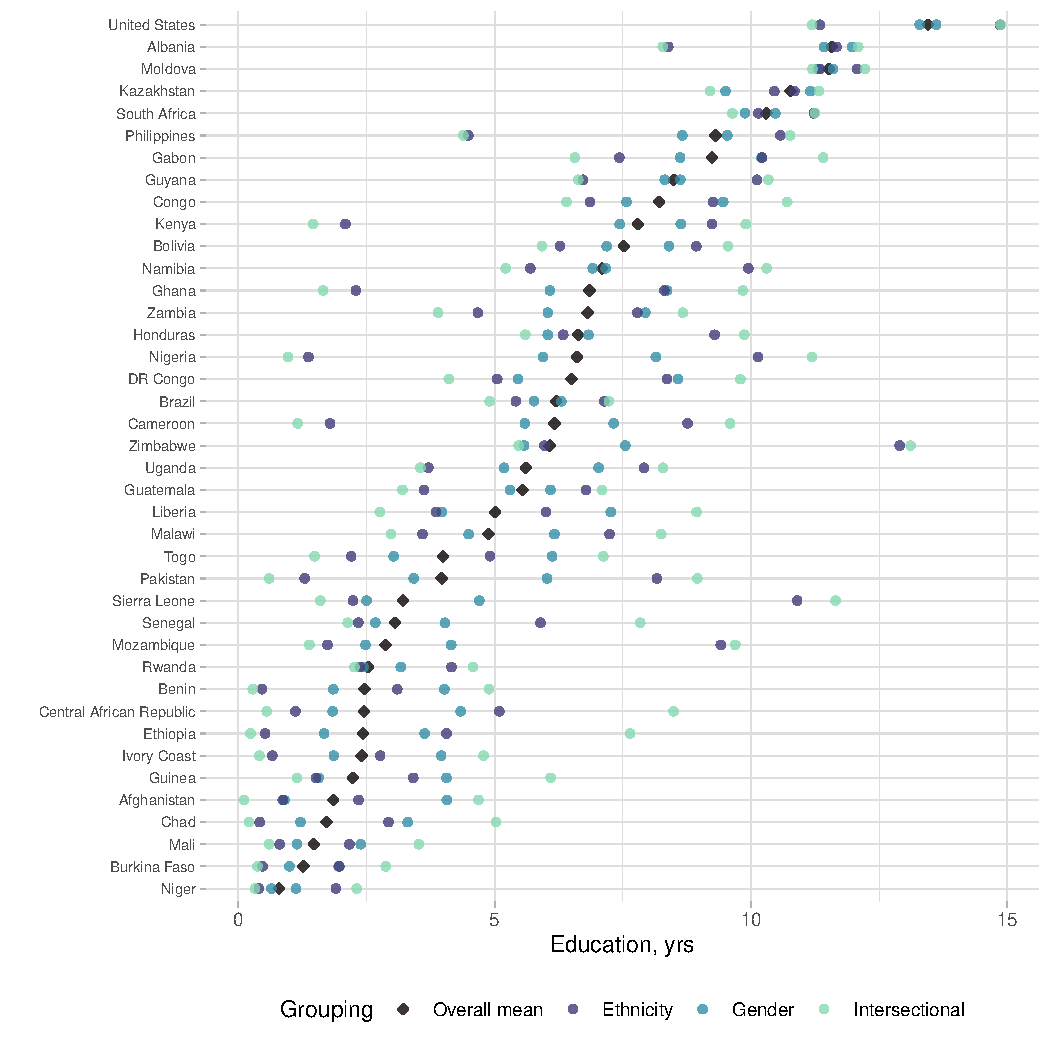
\includegraphics{figures/mean-educ.pdf} \caption[Average Years in Education by Group]{Average Years in Education by Group}\label{fig:mean-educ}
\floatfoot{\textit{Notes:} 
Pooled data from 40 countries; $n=$2,689,279 individuals older than 25 years and younger than the birth cohort of 1920. Estimates to the right of the overall mean represent the average education of the group with the highest education. Means are calculated using DHS sample weights. Sources: DHS 1992-2019 and US CPS 2019.
} \end{figure}

\clearpage

\hypertarget{robustness-checks-with-the-theil-index}{%
\section{Robustness Checks}\label{robustness-checks-with-the-theil-index}}
\setcounter{table}{0}
\renewcommand{\thetable}{\thesection\arabic{table}}

Alternatively to the inequality ratio \(IR\) we can use a variant of the Theil Index, which is a special case of the General Entropy measures, as follows:

\[
T(G) = \frac{1}{J}\sum_{j=1}^{J}\frac{s_j}{\mu_s}arsinh(\frac{s_j}{\mu_s}),
\]

where \(s_j\) denotes the group averages, as previously defined for \(IR\), \(J\) denotes the numbers of groups and \(\mu\) the unweighted mean of all \(s_j\). Instead of the natural logarithm, as is normally used for the Theil Index, we use an inverse hyperbolic sine transformation (\(arsinh\)). It has the advantage of being defined for zero values, which is a problem that we would inevitably run into with education data from low- and middle-income countries.

Repeating the regressions shown in Table \ref{tab:ratios}, but with inequality measured by the Theil Index instead of the inequality ratio leads to the results reported in Table \ref{tab:theil}. The results remain fairly comparable.

\begin{table}

\caption{OLS Regression of Between-Group Theil Indices of Education Inequality\label{tab:theil}}
\centering
\begin{tblr}[         %% tabularray outer open
]                     %% tabularray outer close
{                     %% tabularray inner open
colspec={Q[]Q[]Q[]Q[]},
cell{1}{2}={c=3,}{halign=c,},
column{1}={halign=l,},
column{2}={halign=c,},
column{3}={halign=c,},
column{4}={halign=c,},
hline{21}={1,2,3,4}{solid, 0.05em, black},
}                     %% tabularray inner close
\toprule
& Group Theil Index &  &  \\ \cmidrule[lr]{2-4}
& (A) & (B) & (C) \\ \midrule %% TinyTableHeader
Mean education (yrs)$^a$ & -0.02245*** &            &            \\
& (0.00352)   &            &            \\
No. of ethnic groups     &             & 0.00296    &            \\
&             & (0.00439)  &            \\
Sample size$^b$          &             & -0.00011*  &            \\
&             & (0.00006)  &            \\
Group size lowest        &             &            & -0.00001*  \\
&             &            & (0.00000)  \\
Group size highest       &             &            & 0.00000    \\
&             &            & (0.00001)  \\
Africa                   & -0.02086    & 0.03890    & 0.05458    \\
& (0.02329)   & (0.04250)  & (0.03524)  \\
Cohort 1970-1979$^c$     & -0.00260    & -0.01576   & -0.01250   \\
& (0.00796)   & (0.01020)  & (0.01128)  \\
Cohort 1980-$^c$         & 0.00106     & -0.02475*  & -0.01974   \\
& (0.00965)   & (0.01266)  & (0.01356)  \\
(Intercept)              & 1.12170***  & 0.94132*** & 0.95245*** \\
& (0.03680)   & (0.02742)  & (0.03487)  \\
Adj. R2                  & 0.555       & 0.061      & 0.055      \\
Num.Obs                  & 105         & 105        & 105        \\
\bottomrule
\end{tblr}

\floatfoot{\textit{Notes:} Aggregated country-cohort bracket level data from 40 countries; n=2'689'279 individuals 25 years and older, and born after 1920; cluster-robust standard errors on the country-level in parentheses; Sign. codes: $^*p<10\%$, $^{**}p<5\%$, $^{***}p<1\%$. \\
$^a$~Within-country-cohort weighted mean years of education with DHS sampling weights;\\
$^b$~Within-country-cohort (individual) Gini index takes on a value between 0 and 1;\\
$^c$~Corresponds to country-cohort sample size in units of 1000;\\
$^d$~Ref: Cohort -1969.}
\end{table}